\begin{table}[H]
\centering
\begin{tabularx}{\linewidth}{@{}>{\centering\arraybackslash}m{3cm}>{\centering\arraybackslash}X>{\centering\arraybackslash}X>{\centering\arraybackslash}X@{}}
\toprule
 & Image 1 & Image 2 & Image 3 \\
\midrule
Original\newline Dataset & 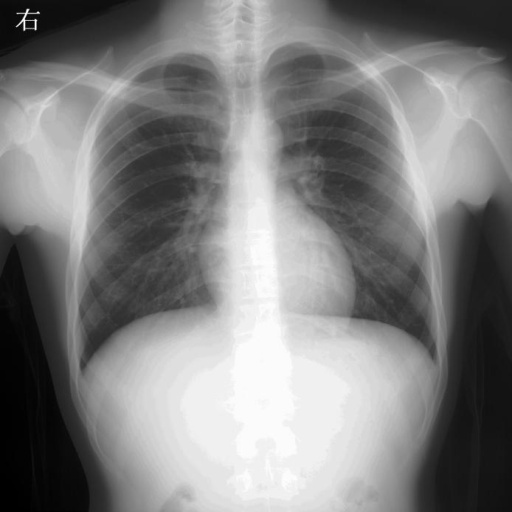
\includegraphics[valign=M,width=\linewidth,height=4cm,keepaspectratio]{main/content/images/pggan/original_dataset/56286.jpg} & 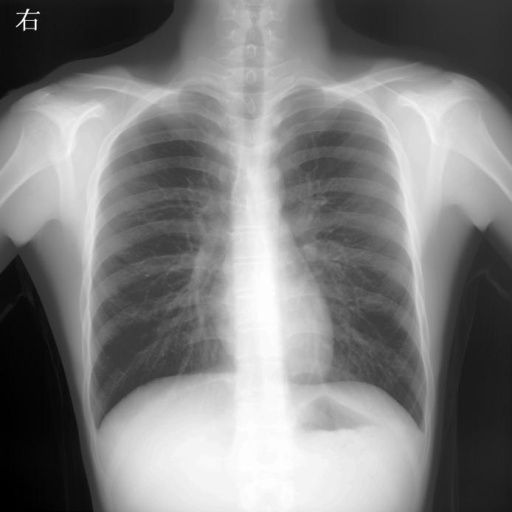
\includegraphics[valign=M,width=\linewidth,height=4cm,keepaspectratio]{main/content/images/pggan/original_dataset/56287.jpg} & 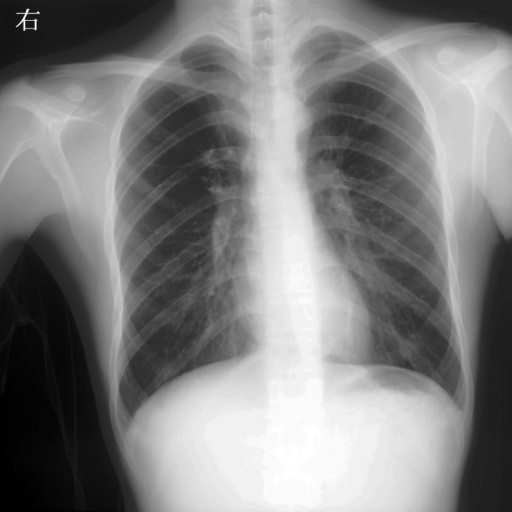
\includegraphics[valign=M,width=\linewidth,height=4cm,keepaspectratio]{main/content/images/pggan/original_dataset/56289.jpg} \\
\midrule
PGGAN & 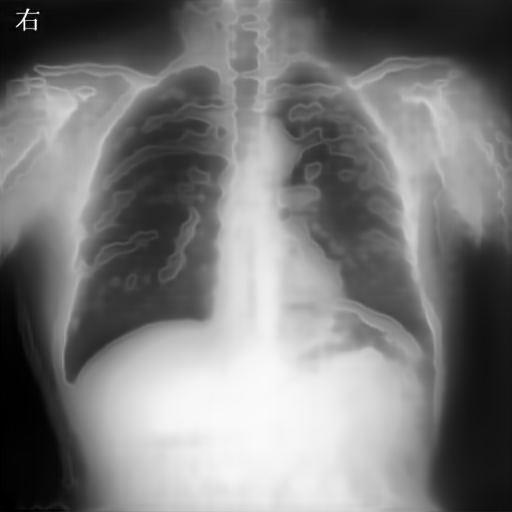
\includegraphics[valign=M,width=\linewidth,height=4cm,keepaspectratio]{main/content/images/pggan/train_pneumoconiosis/111.png} & 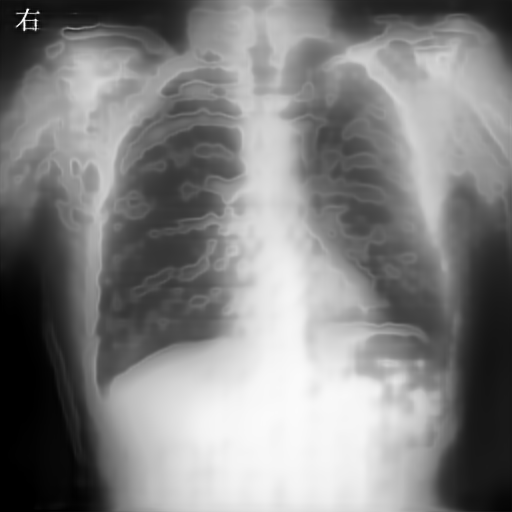
\includegraphics[valign=M,width=\linewidth,height=4cm,keepaspectratio]{main/content/images/pggan/train_pneumoconiosis/112.png} & 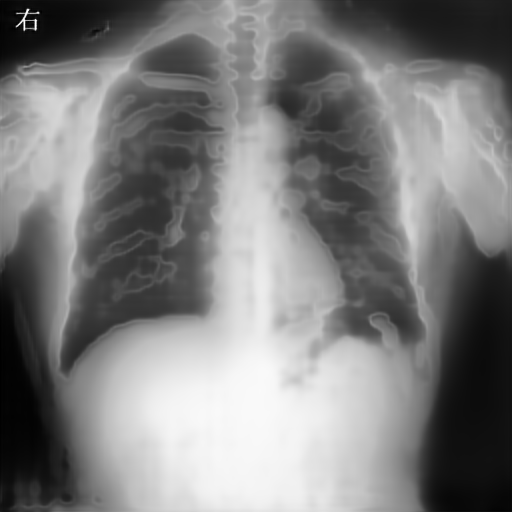
\includegraphics[valign=M,width=\linewidth,height=4cm,keepaspectratio]{main/content/images/pggan/train_pneumoconiosis/113.png} \\
\midrule
PGGAN with\newline NIH Chest X-ray\newline Fine-Tuning & 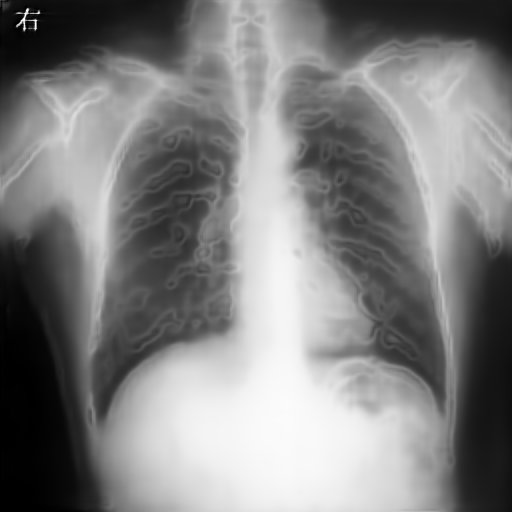
\includegraphics[valign=M,width=\linewidth,height=4cm,keepaspectratio]{main/content/images/pggan/train_pneumo_finetuned_chestxray/111.png} & 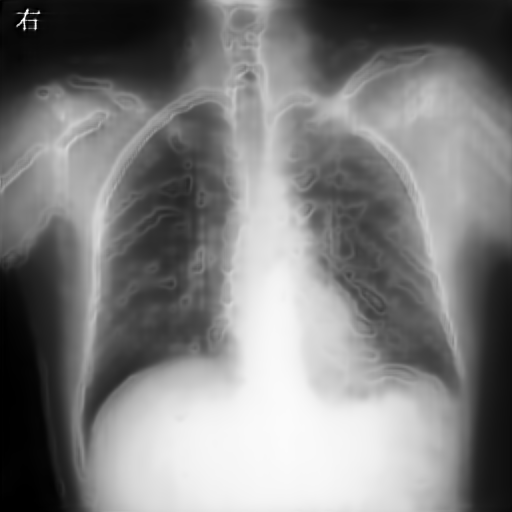
\includegraphics[valign=M,width=\linewidth,height=4cm,keepaspectratio]{main/content/images/pggan/train_pneumo_finetuned_chestxray/112.png} & 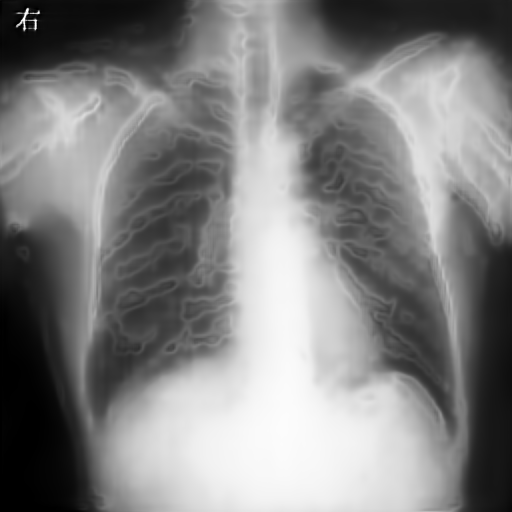
\includegraphics[valign=M,width=\linewidth,height=4cm,keepaspectratio]{main/content/images/pggan/train_pneumo_finetuned_chestxray/113.png} \\
\bottomrule
\end{tabularx}
\caption{Comparison of original images (a, b, c) with those generated using PGGAN (d, e, f) and PGGAN fine-tuned with chest X-ray images (g, h, i) based on the different types of noise added.}
\label{tab:image_comparison_pggan}
\end{table}
